%preamble
\documentclass[letterpaper]{article}
\synctex=1
\usepackage{graphicx}
\graphicspath{ {images/} }

\usepackage{lipsum}
\usepackage{float}
% \bibliographystyle{IEEEtran}
% \bibliographystyle{ieeetr}

\usepackage{amssymb}

\usepackage{siunitx}

\usepackage{multirow}
% for merging table cells I think

% make subsection use letters
\renewcommand{\thesubsection}{\thesection.\alph{subsection}}

%actual document
\begin{document}

% \maketitle %insert titlepage here
\begin{titlepage}
 \begin{center}
  \vspace*{1cm}
  \Huge
  Stat 235
  \vspace{1cm}

  Lab 1
  \vspace{1cm}

  By: Arun Woosaree
  \vspace{1cm}

  \Huge
  Lab EL12
  \vspace{1cm}

  TA: Jessa Marley
  \vspace{1cm}

  \today
  \vfill
 \end{center}
\end{titlepage}

\section{Histograms}

  \subsection{Histograms of Thickness: 400ºC, 600ºC, and 800ºC}

    \begin{figure}[H]
      \centering
      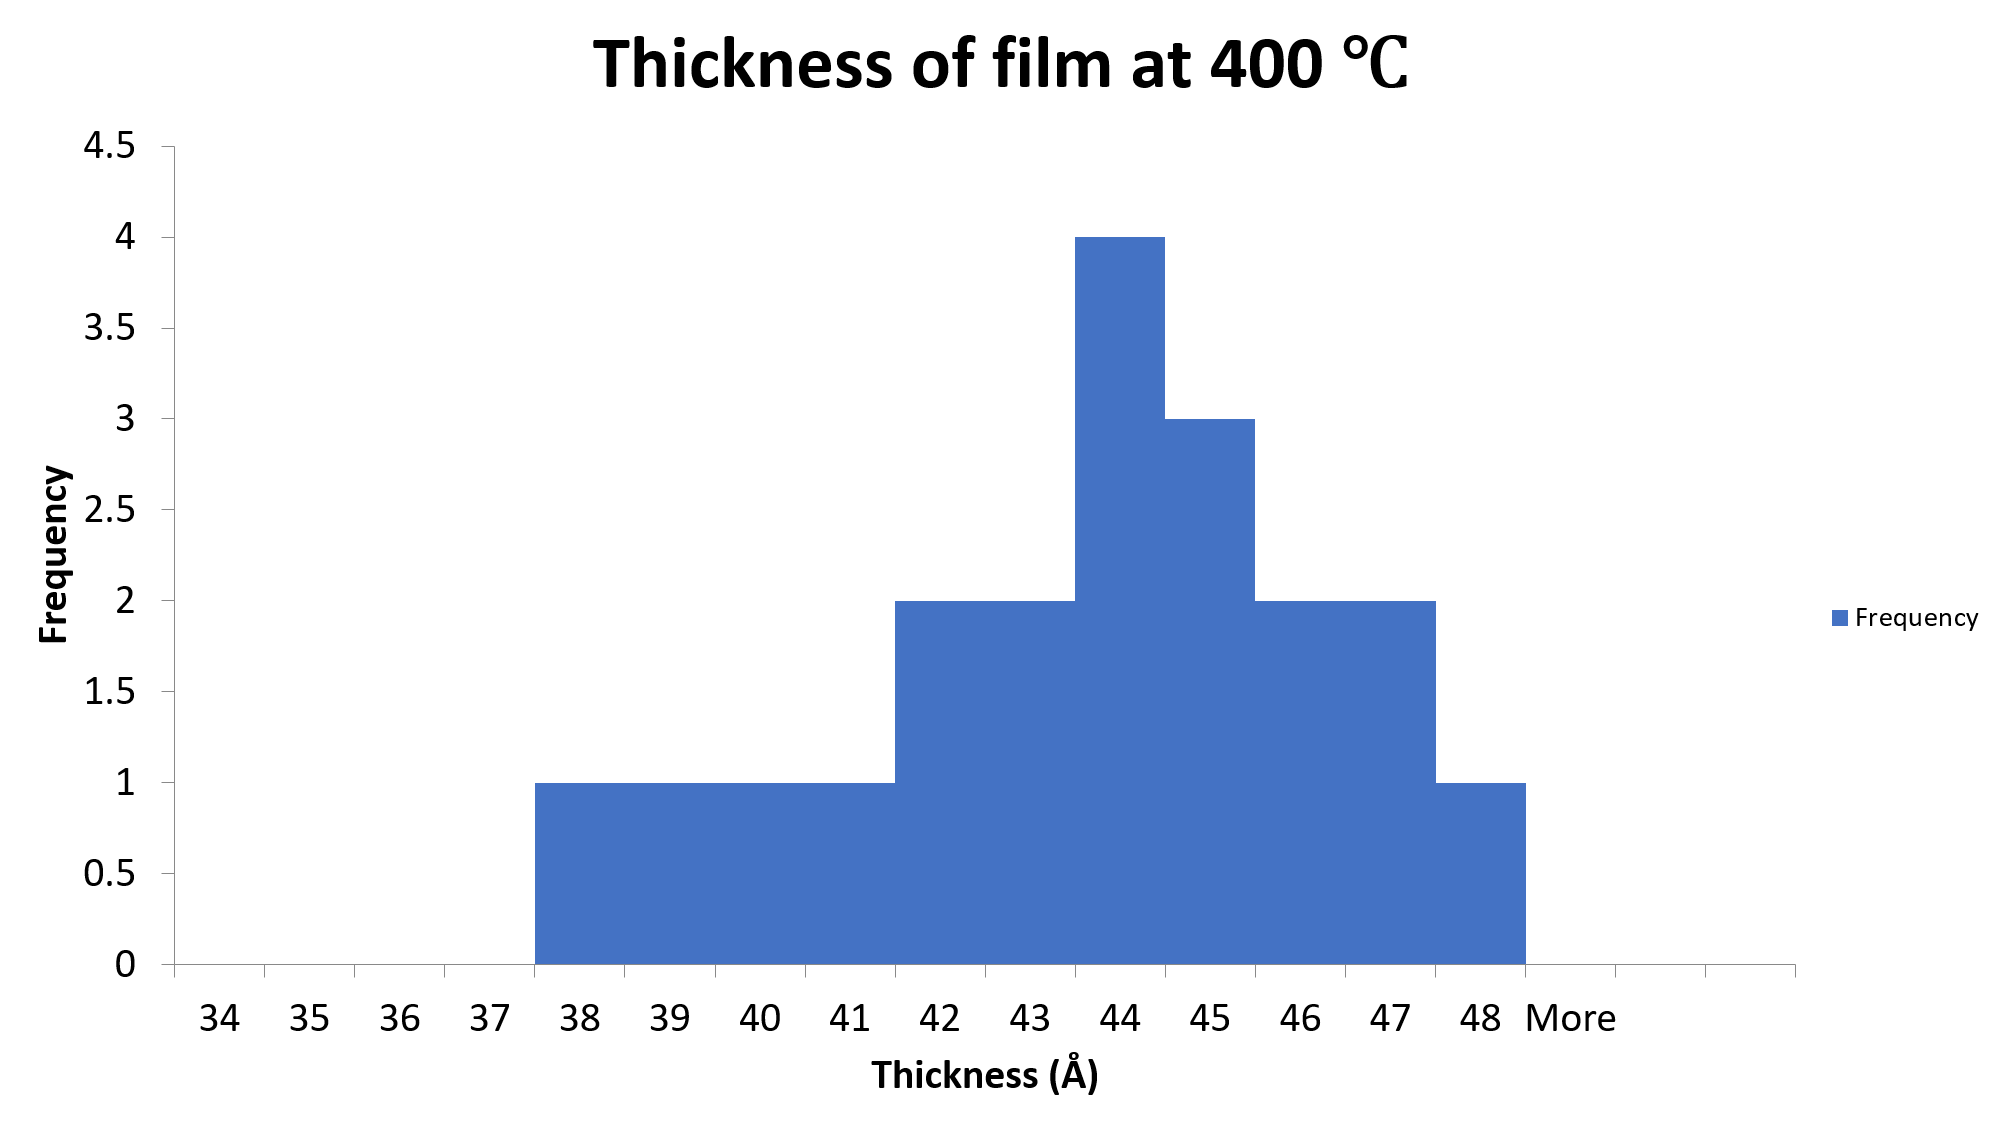
\includegraphics[width=\textwidth]{thicc400.png}
      \caption{INSERT CAPTION HERE}
      \label{thicc400}
    \end{figure}

    \begin{figure}[H]
      \centering
      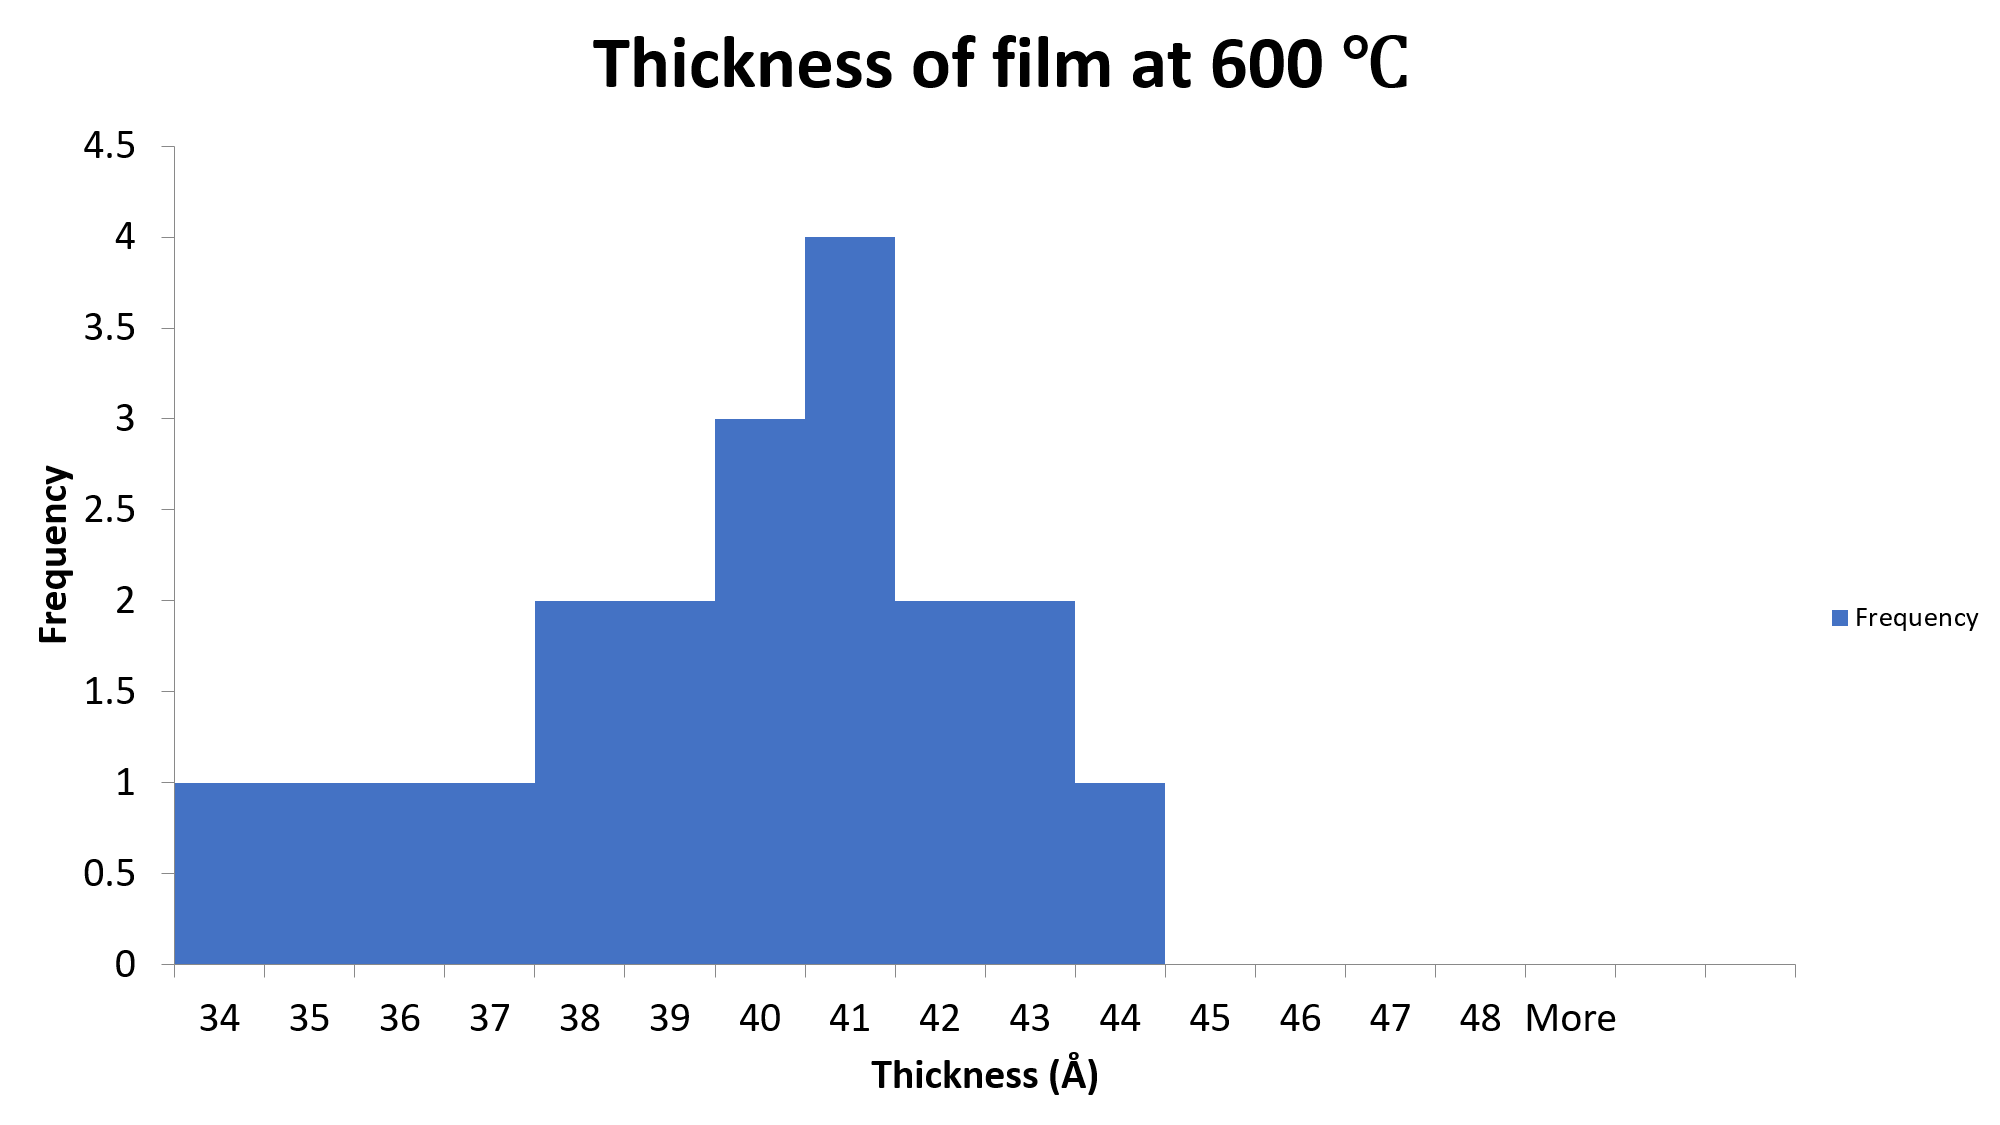
\includegraphics[width=\textwidth]{thicc600.png}
      \caption{INSERT CAPTION HERE}
      \label{thicc600}
    \end{figure}

    \begin{figure}[H]
      \centering
      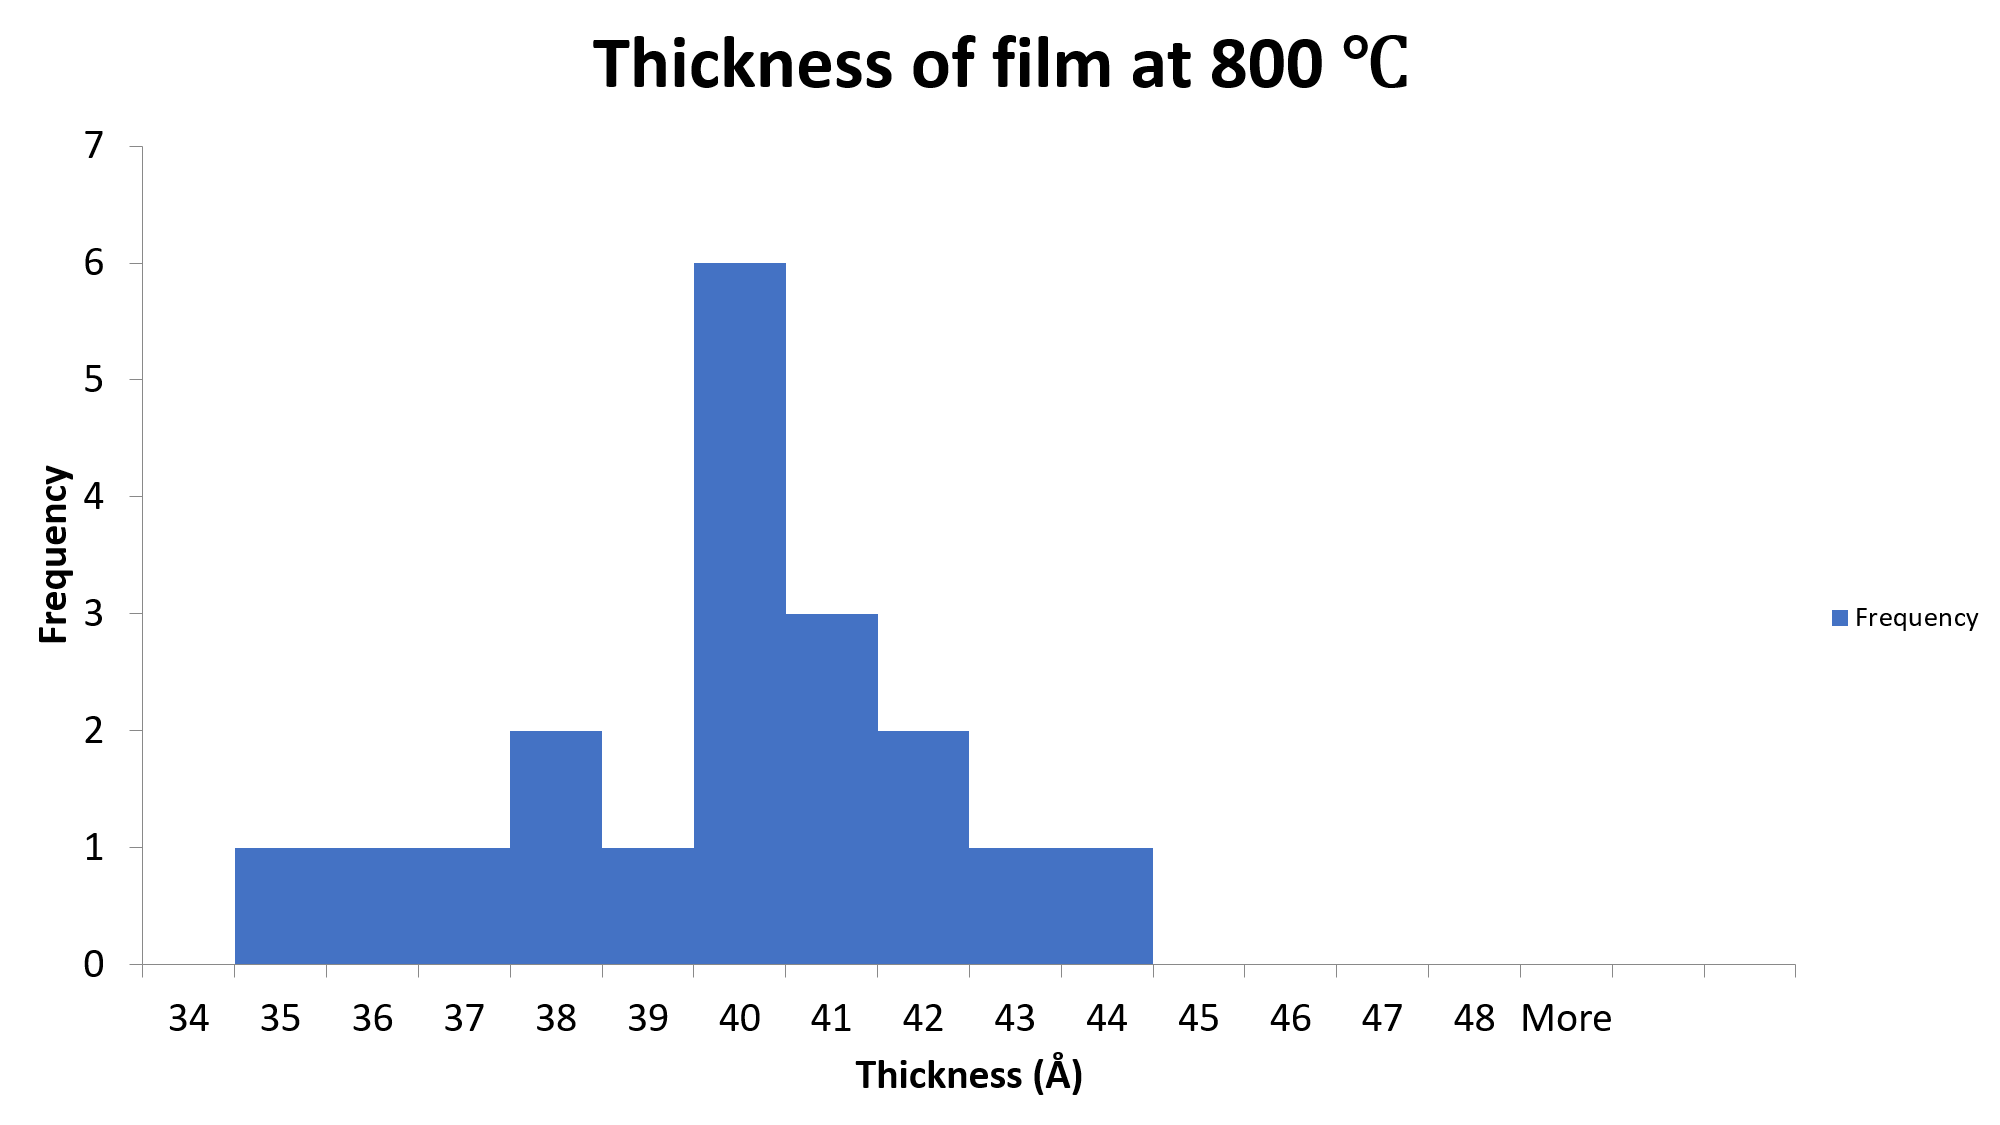
\includegraphics[width=\textwidth]{thicc800.png}
      \caption{INSERT CAPTION HERE}
      \label{thicc800}
    \end{figure}

  \subsection{Shapes}
    All the histograms above appear to be slightly left-skewed.
    By simply looking at the histograms, only one peak is observable in each of them, therefore all the histograms above are single-peaked
    There don’t seem to be any obvious outliers judging from the 3 histograms above. At first glance, the one data point that has a thickness of 33  at 800  may seem like a potential outlier, but when looking at the bigger picture in the histogram, we can see that it (in bin 34) is not visually far away from the bulk of the data

  \subsection{Centers and Spreads}
    The first histogram has a center around 44, and a spread of 10.
    The second histogram has a center about 42 and a spread of 10 as well.
    The third histogram has a center around 40, and also has a spread of 10.
    For all 3 histograms, the means are slightly less than their respective medians.


  \subsection{Effect of Temperature on Thickness}
    It would appear that increased temperature results in an overall lower average of thickness of the films.

\section{Summary Statistics}

  \subsection{Mean, Std. Deviation, Variance for each Temperature Level}

    \begin{table}[H]
    \centering
    \begin{tabular}{c|c|c|c|}
    \multirow{2}{*}{Statistics} & \multicolumn{3}{c|}{Temperature Levels (\SI{}{\celsius})} \\ \cline{2-4}
                                & 400           & 600          & 800          \\ \hline
    Mean                        & 0             & 0            & 0            \\ \hline
    Std. Deviation              & 0             & 0            & 0            \\ \hline
    Variance                    & 0             & 0            & 0            \\ \hline
    \end{tabular}
    \caption{My caption}
    \label{tempmean}
    \end{table}


  \subsection{Quartiles}

    \begin{table}[H]
    \centering
    \begin{tabular}{c|c|c|c|}
    \multirow{2}{*}{Statistics} & \multicolumn{3}{c|}{Temperature Levels (\SI{}{\celsius})} \\ \cline{2-4}
                                & 400           & 600          & 800          \\ \hline
    Lower Quartile              & 0             & 0            & 0            \\ \hline
    Median                      & 0             & 0            & 0            \\ \hline
    Upper Quartile              & 0             & 0            & 0            \\ \hline
    IQR                         & 0             & 0            & 0            \\ \hline
    \end{tabular}
    \caption{My caption}
    \label{tempquart}
    \end{table}

    Wait check this
    The 400  one doesn’t seem to match, but for 600  and 800 , the positions of the quartiles seem to support the conclusion that these histograms are left-skewed, since Q1 is further from the median than Q3 is.
  \subsection{Mean \& Std. Deviation at each pressure value}

    \begin{table}[H]
    \centering
    \begin{tabular}{c|c|c|c|}
    Pressure & Mean & Std. Deviation & Mean Change \\ \hline
    0        & 0    & 0              & 0           \\ \hline
    Average  &      &                & 0           \\ \hline
    \end{tabular}
    \caption{My caption}
    \label{pressurestat}
    \end{table}

\section{Relationships}

  \subsection{Thickness vs. Temperature}

    \begin{figure}[H]
      \centering
      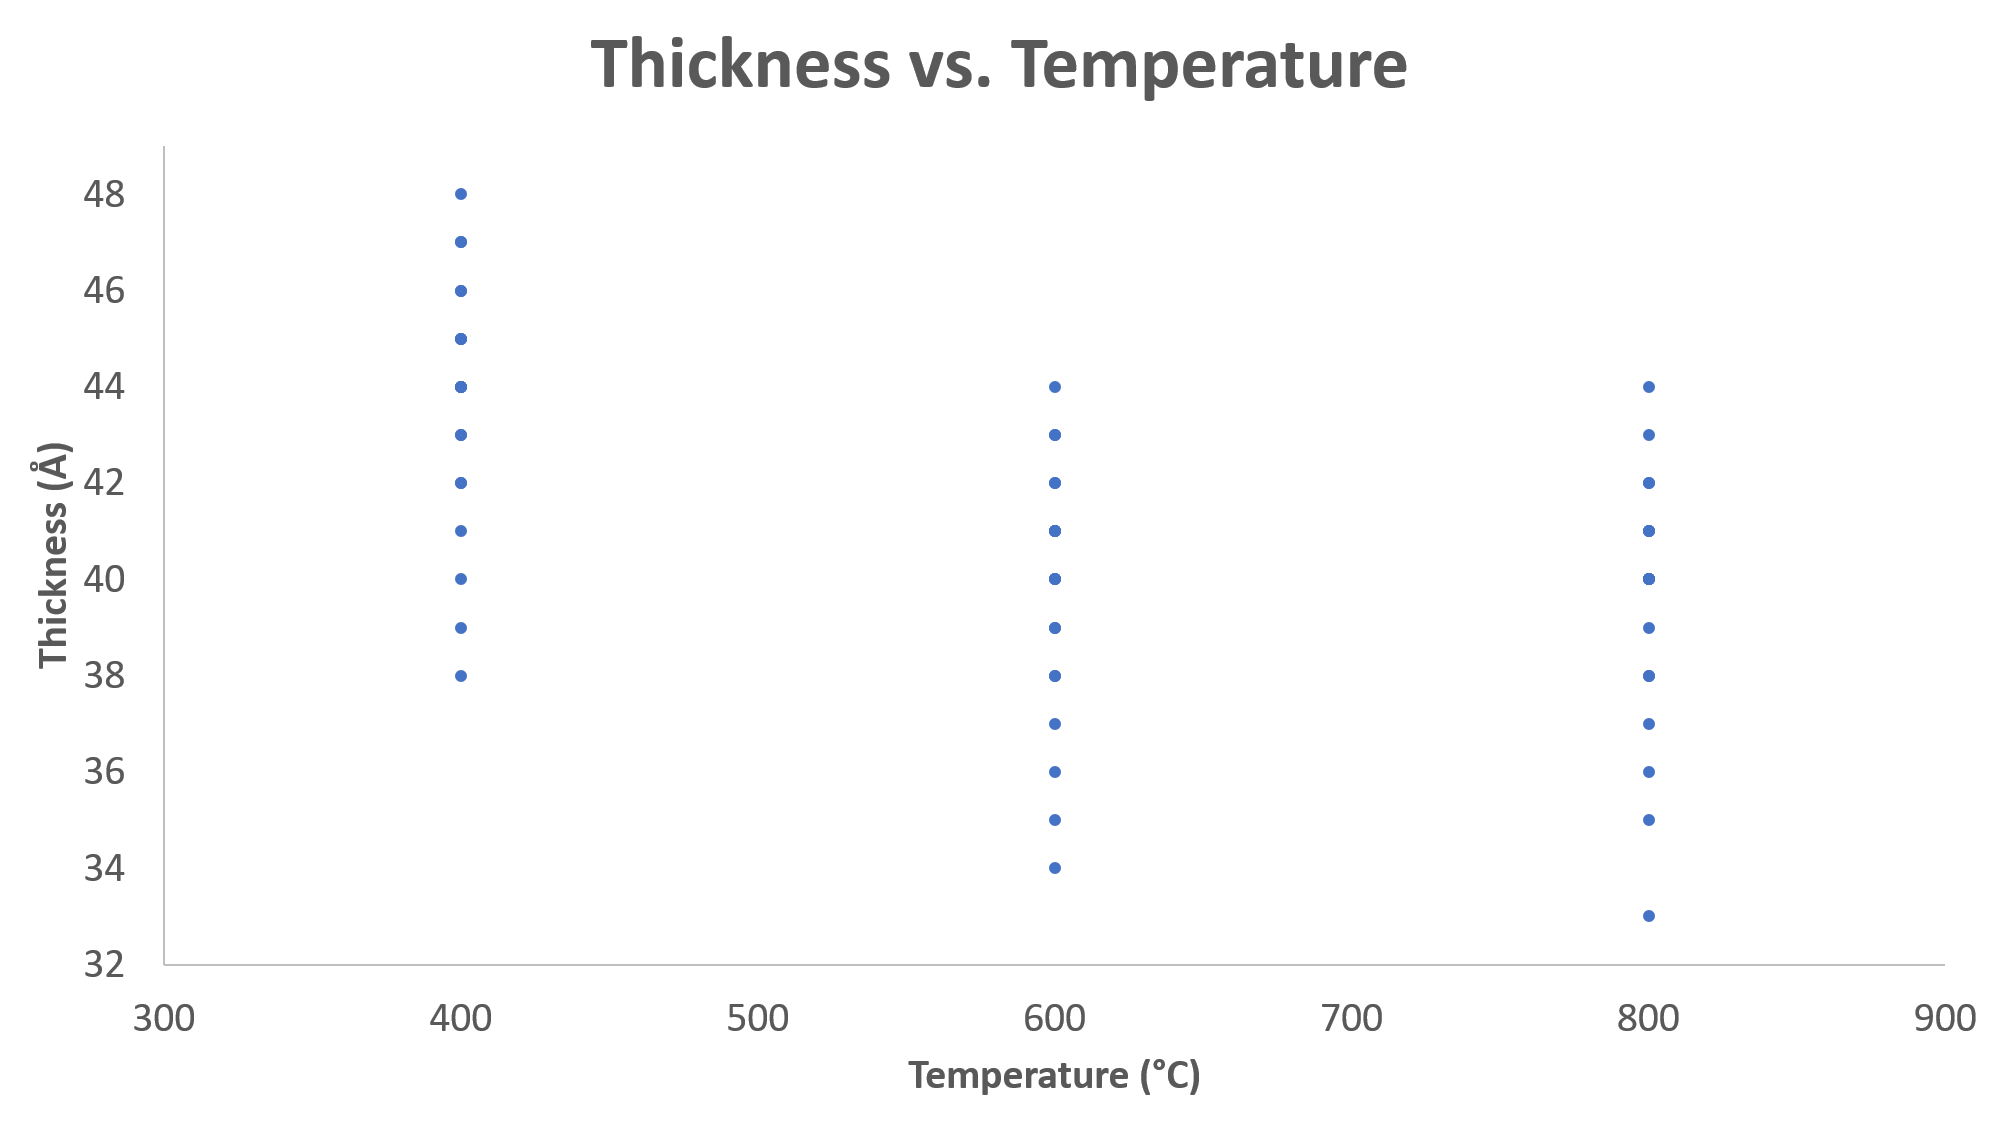
\includegraphics[width=\textwidth]{thiccvstemp.png}
      \caption{INSERT CAPTION HERE}
      \label{thiccvstemp}
    \end{figure}

  \subsection{Thickness vs. Pressure by Temperature}

    \begin{figure}[H]
      \centering
      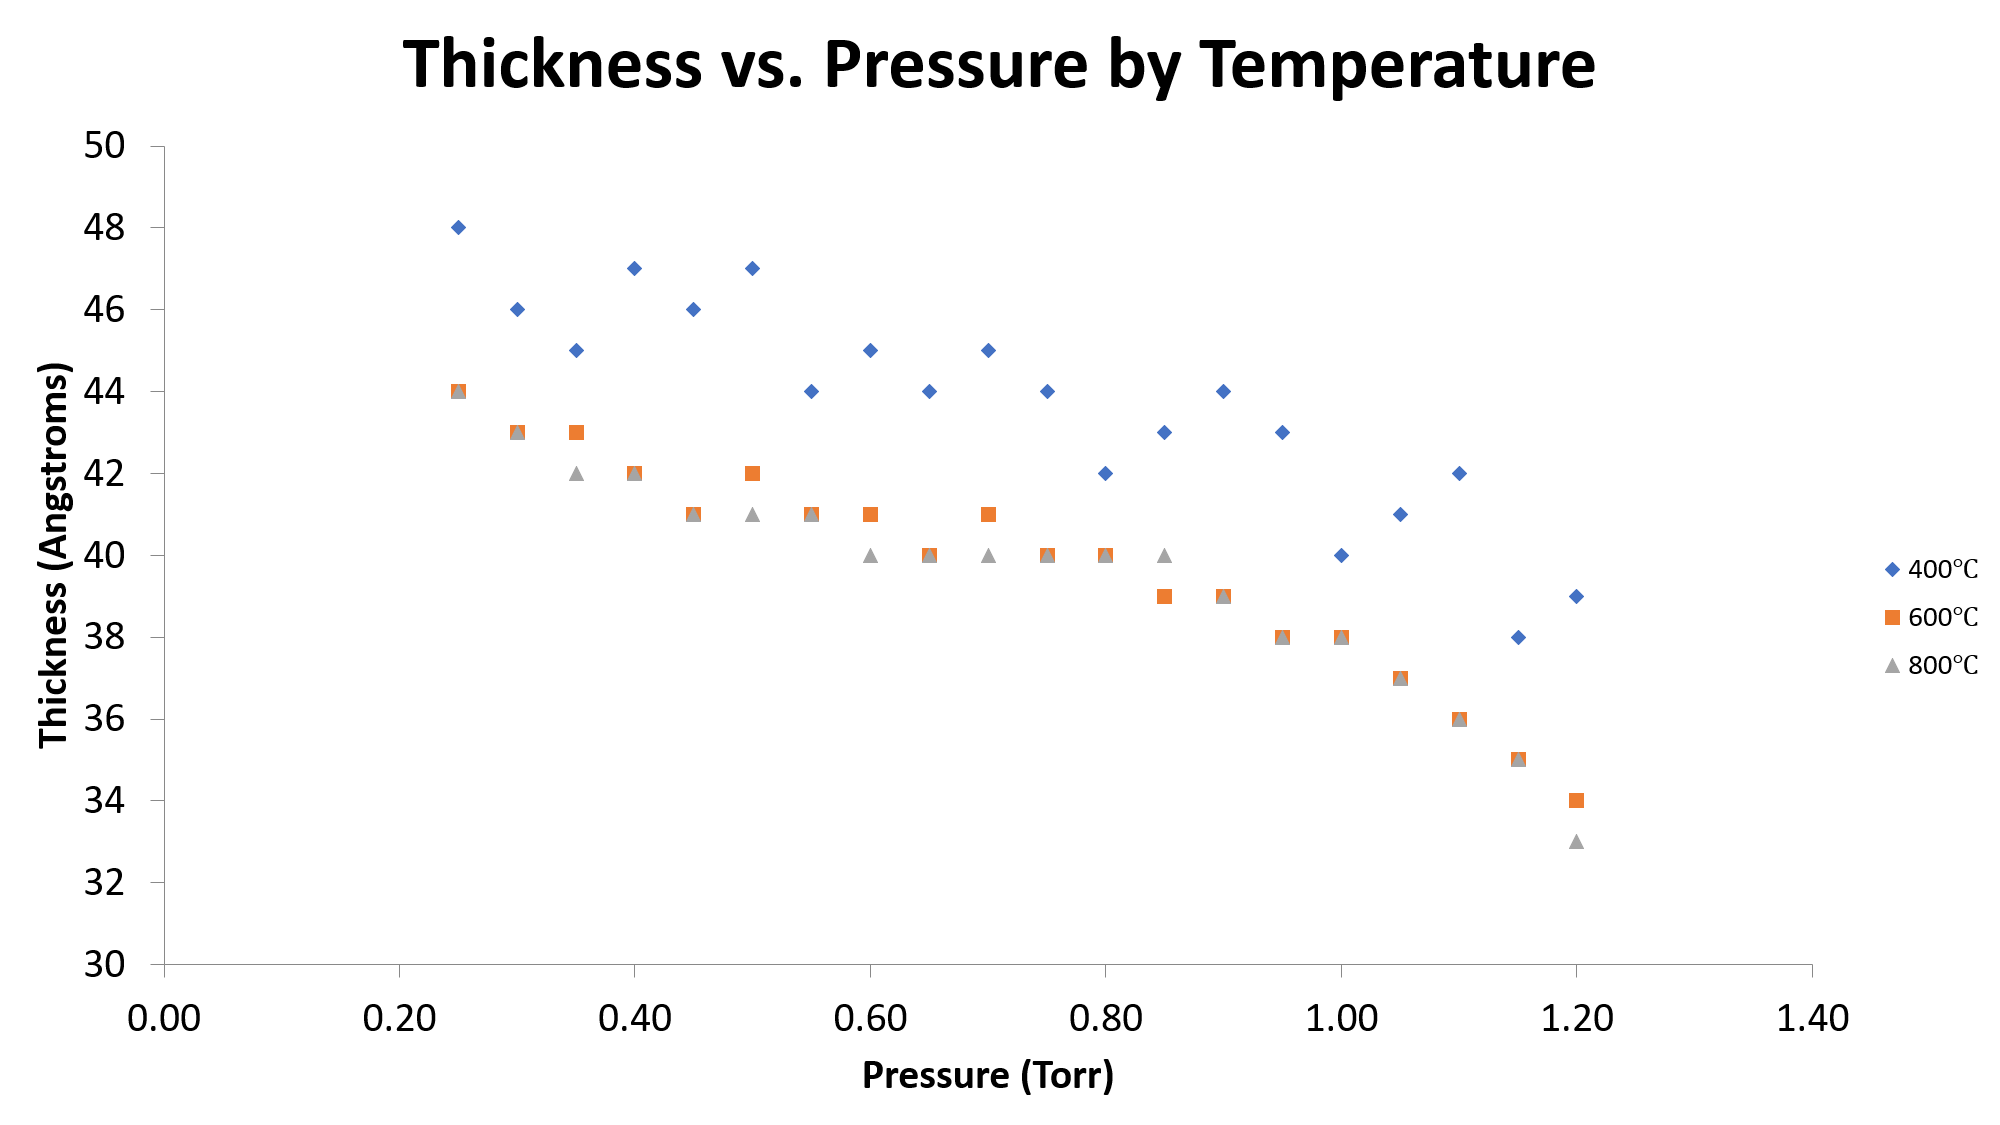
\includegraphics[width=\textwidth]{thiccvspressurebytemp.png}
      \caption{INSERT CAPTION HERE}
      \label{thiccvspressurebytemp}
    \end{figure}


  \subsection{Relationship Between Thickness and Pressure for each Temperature Level}

\section{How should the temperature and pressure be selected to produce the thinnest possible film for the LPCVD
process?}





\end{document}
